\section{Evolução estocástica por complexos}

\missingt{Justificar o uso do SCE.}

O Algoritmo de Evolução estocástica por complexos (EEC),
\emph{Shuffled Complex Evolution} em inglês,
é um algoritmo evolutivo populacional proposto por Duan~\cite{duan1992effective}
e tem sido utilizado com sucesso em problemas de escalonamento
\cite{zhao2015shuffled}, seleção de projetos~\cite{elbeltagi2007modified},
problema da mochila $0-1$~\cite{bhattacharjee2014shuffled} e
problema da mochila multi-dimensional~\cite{baroni2015shuffled,baroni2016shuffled}.

O EEC é inspirado na evolução natural que ocorre de forma simultânea em
comunidades independentes.
O algoritmo trabalha com uma população particionada em $N$ comunidades,
ou complexos, cada uma contendo $M$ indivíduos.
Inicialmente a população de $N*M$ indivíduos é tomada aleatoriamente do espaço
de soluções viáveis.
Após esta inicialização a população é ordenada em ordem descrecente de aptidão
e o melhor global é identificado.
Toda a população é então particionada em $N$ complexos, cada um contendo $M$ indivíduos.
Neste processo de distribuição aleatória o primeiro indivíduo é incluído
no primeiro complexo, o segundo indivíduo no segundo complexo, o $M$-ésimo
indivíduo no $M$-ésimo complexo, o $M+1$-ésimo indivíduo no primeiro complexo,
e assim por diante.

O próximo passo após a distribuição dos indivíuos em complexos é evoluir cada
complexo uma quantidade constante $K'$.
Neste processo, considerando que os indivíduos em cada complexo estão ordenados
em ordem decrescente de aptidão, um subcomplexo é de $P$ indivíduos é selecionado
dentre o complexo utilizando uma distribuição triangular, em que o $i$-ésimo
indivíduo tem a probabilidade $p_i = \frac{2(n+1-i)}{n(n+1)}$ de ser selecionado.
A utilização da distribuição triangular tem por objetivo priorizar os indivíduos
com melhor aptidão, favorecendo assim a convergência do algoritmo.

Após a seleção do subcomplexo, o seu pior indivíduo é identificado para ser
subtituido por um novo indivíduo.
Este novo indivíduo é gerado através do cruzamento do pior indivíduo e um outro
indivíduo com melhor aptidão.
Primeiramente o melhor indivíduo do subcomplexo é considerado.
Caso o indivíduo gerado não seja melhor que o pior indivíduo selecionado,
o melhor indivíduo do complexo é então usado no cruzamento.
Se este último cruzamento não resultou em melhoria, o melhor indivíduo de toda
a população é considerado.
Finalmente, se todos os cruzamentos não foram capaz de gerar um melhor indivíduo,
esta pior solução selecionada é substituída por um novo indivíduo retirado de
forma aleatória do espaço de soluções viáveis.
Este último procedimento é importante para impedir que o algoritmo fique
\emph{preso} num ótimo local.
A Figura~\ref{img:flow2} apresenta o procedimento de evolução descrito acima
em um fluxograma.

\begin{figure}[]
  \centering
  \begin{minipage}[b]{0.42\textwidth}
    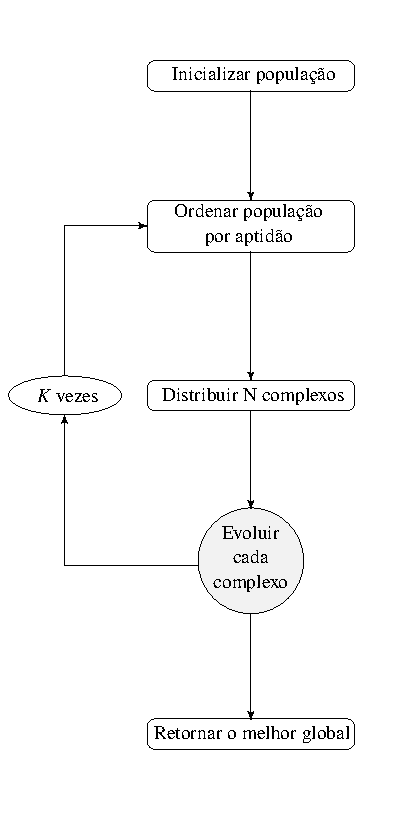
\includegraphics[width=\textwidth]{img/sce/flow1}
    \caption{The shuffled complex evolution algorithm.}
    \label{img:flow1}
  \end{minipage}
  \hfill
  \begin{minipage}[b]{0.42\textwidth}
    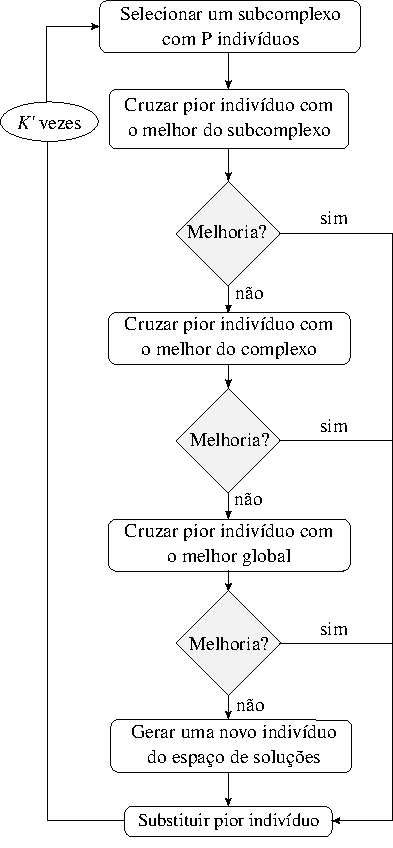
\includegraphics[width=\textwidth]{img/sce/flow2}
    \caption{The evolving stage of SCE for a single complex.}
    \label{img:flow2}
  \end{minipage}
\end{figure}

Após evoluir todos os $N$ complexos toda a população é novamente ordenada
em ordem descrecente de aptidão e o processo continua até que a condição
de parada seja satisfeita.

A Figura~\ref{img:flow1} apresenta os passos do algoritmo ECC num fluxograma
em que a condição de parada é a execução de uma quantidade fixa de $K$ evoluções.


\section{O EEC para o MOKP}
Como pode-se notar em sua descrição, o EEC é facilmente aplicável a qualquer
problema de otimização, inclusive o MOKP, desde que seja possível (a) definir
um procedimento de criação de uma nova solução alteatória viável e (b) definir
um procedimento de cruzamento entre duas soluções.
Esses dois procedimentos para o MOKP são descritos no Algoritmo~\ref{alg:new}
e Algoritmo~\ref{alg:cross}.

\begin{algorithm}
  \Begin{
  $v \leftarrow $ shuffle($1, 2, \ldots, n$)\;
  $s \leftarrow \vec{0}$; \Comment{solução vazia}\\
  \For{$ i \leftarrow 1:n$ }{
    $s[v_i] \leftarrow 1$; \Comment{inserção de item}\\
    \If{ $w(s) > W$ }{
      $s[v_i] \leftarrow 0$; \Comment{verificação de viabilidade}\\
    }
  }
  \textbf{retorna} $s$\;
}
  \caption{Construção de solução aleatória para o MOKP.}
  \label{alg:new}
\end{algorithm}

Para se contruir uma nova solução aleatória para o MOKP (Algoritmo~\ref{alg:new})
os índices dos $n$ itens são primeiramente permutados em ordem aleatória e
armazenados em uma lista $v$ (linha 2).
Uma nova solução vazia é definida (linha 3).
O algoritmo tenta de forma iterativa preencher a solução com um item retirado
da lista de índices (linhas 4-9).
A viabilidade da solução é então verificada: se o item inserido tornar a solução
inviável (linha 6) ele é então retirado da solução (linha 7).
Após testar a inserção de todos os itens a solução contruida é retornada.

\begin{algorithm}
  \Kw{$x:$ pior indivíduo, $y:$ melhor indivíduo, $c$: número de genes herdados}
\Begin{
  $v \leftarrow $ shuffle($1, 2, \ldots, n$)\;
  $z \leftarrow \ord^{max}_{rev}$\;
  \For{$i \leftarrow 1:c$ }{
	  $x[v_i] \leftarrow y[v_i];$\ \Comment{herança de genes}
  }
  \For{$i \gets 1:n$ \textbf{and} $w(x) > W$}{
    $x[z_i] \gets 0;$\ \Comment{reparo de solução}
  }
	Computar aptidão de $x$\;
  \textbf{return} $x$\;
}
  \caption{Procedimento de cruzamento entre duas soluções do MOKP.}
  \label{alg:cross}
\end{algorithm}


O procedimento de cruzamento (Figura~\ref{alg:cross}) recebe como entrada
$s$ o pior indivíduo vindo do subcomplexo selecionado, $b$ um indivíduo com
maior aptidão que $s$ e parâmetro $c$ sendo o número de genes a serem carregados de $b$.
O parâmetro $c$ controla o quão similar o novo indivíduo será do melhor indivíduo
dado como entrada.
Primeiramente os índices dos $n$ itens são permutados em uma ordem aleatória e armazenados numa lista
(linha 2).
Os $c$ genes escolhidos aleatoriamente é então carregado do melhor indivíduo para
o pior indivíduo (linhas 4-6).
Em seguida a solução é reparada se necessário (linha 6-8).
Finalmente a aptidão da solução gerada é atualizada (linha 8) e então retornada (linha 9).

\missing{Explicar adaptação da heurística para caso multi-objetivo (uso de archive).}
